\documentclass[12pt]{article}
\usepackage[margin=1in]{geometry}
\setlength{\headheight}{14.49998pt}
\usepackage{graphicx}
\usepackage{float}
\usepackage{amsmath}
\usepackage{amsfonts}
\usepackage{amssymb}
\usepackage{xcolor}
\usepackage{url}
\usepackage{hyperref}
\usepackage{fancyhdr}
\usepackage{titlesec}
\titlelabel{}
\renewcommand{\thesection}{}
\renewcommand{\thesubsection}{}
\renewcommand{\thesubsubsection}{}
\setcounter{secnumdepth}{0}

\pagestyle{fancy}
\fancyhf{}
\rhead{Cameron Brooks}
\lhead{CS321 Assignment 5}
\cfoot{\thepage}

\titleformat{\section}{\Large\bfseries}{\thesection}{1em}{}
\titleformat{\subsection}{\large\bfseries}{\thesubsection}{1em}{}
\titleformat{\subsubsection}{\normalsize\bfseries}{\thesubsubsection}{1em}{}

\title{Assignment 5: Context-Free Grammars, Parsing, and Ambiguity}
\author{Cameron Brooks \\
        CS321 Introduction to Theory of Computation \\
        Assignment 5}
\date{Wednesday, October 31, 2025}

\begin{document}

\maketitle
\thispagestyle{empty}

\newpage
\tableofcontents
\newpage

\section{Section 5.1: Context-Free Grammar Construction}

\subsection{Problem 1: CFG for $L = \{a^n b^m : 2n \le m \le 3n\}$}

\subsubsection{Problem Statement}
Create a context-free grammar for the language $L = \{a^n b^m : 2n \le m \le 3n\}$.

\subsubsection{Solution}

\textbf{Context-Free Grammar:}

$$S \rightarrow aSbb \mid aSbbb \mid \lambda$$

\subsubsection{Explanation}

The constraint $2n \le m \le 3n$ requires that for each $a$ in the string, there must be at least 2 $b$'s and at most 3 $b$'s. The grammar achieves this by allowing each recursive step to choose between adding 2 or 3 $b$'s for every $a$ generated.

The production $S \rightarrow aSbb$ generates one $a$ followed by exactly 2 $b$'s, then recurses to generate more. The production $S \rightarrow aSbbb$ generates one $a$ followed by exactly 3 $b$'s, then recurses. The base case $S \rightarrow \lambda$ generates the empty string when $n=0$ and $m=0$. By mixing these two recursive rules in any combination, we can generate any value of $m$ in the range $[2n, 3n]$ for a given $n$.

\subsubsection{Sample Derivations}

\textit{Example 1: $n=1, m=2$}
$$S \Rightarrow aSbb \Rightarrow abb$$
Verification: $2(1) = 2 \le 2 \le 3 = 3(1)$ \checkmark

\textit{Example 2: $n=1, m=3$}
$$S \Rightarrow aSbbb \Rightarrow abbb$$
Verification: $2(1) = 2 \le 3 \le 3 = 3(1)$ \checkmark

\textit{Example 3: $n=2, m=4$ (using minimum rule twice)}
$$S \Rightarrow aSbb \Rightarrow aaSbbbb \Rightarrow aabbbb$$
Verification: $2(2) = 4 \le 4 \le 6 = 3(2)$ \checkmark

\textit{Example 4: $n=2, m=5$ (mixing rules)}
$$S \Rightarrow aSbb \Rightarrow aaSbbbbb \Rightarrow aabbbbb$$
Verification: $2(2) = 4 \le 5 \le 6 = 3(2)$ \checkmark

\textit{Example 5: $n=2, m=6$ (using maximum rule twice)}
$$S \Rightarrow aSbbb \Rightarrow aaSbbbbbb \Rightarrow aabbbbbb$$
Verification: $2(2) = 4 \le 6 \le 6 = 3(2)$ \checkmark

\subsubsection{Formal Proof of Correctness}

\textbf{Claim:} $L(G) = \{a^n b^m : 2n \le m \le 3n\}$

\textbf{Proof:}

\textit{Part 1: ($L(G) \subseteq \{a^n b^m : 2n \le m \le 3n\}$)}

We prove by induction on the number of derivation steps that every string generated by $G$ satisfies the constraint $2n \le m \le 3n$.

\textit{Base case:} If the derivation uses only $S \rightarrow \lambda$, we generate $\lambda = a^0 b^0$. Since $2(0) = 0 \le 0 \le 0 = 3(0)$, the constraint is satisfied.

\textit{Inductive hypothesis:} Assume that any string derived in $k$ or fewer steps has the form $a^{n'} b^{m'}$ where $2n' \le m' \le 3n'$.

\textit{Inductive step:} Consider a derivation of length $k+1$. The first step must be either $S \rightarrow aSbb$ or $S \rightarrow aSbbb$.

Case 1: If $S \Rightarrow aSbb \Rightarrow^* a \cdot a^{n'} b^{m'} \cdot bb = a^{n'+1} b^{m'+2}$, where by the inductive hypothesis $2n' \le m' \le 3n'$, then:
$$2(n'+1) = 2n' + 2 \le m' + 2 \le 3n' + 2 < 3n' + 3 = 3(n'+1)$$
Therefore, the constraint is satisfied.

Case 2: If $S \Rightarrow aSbbb \Rightarrow^* a \cdot a^{n'} b^{m'} \cdot bbb = a^{n'+1} b^{m'+3}$, where $2n' \le m' \le 3n'$, then:
$$2(n'+1) = 2n' + 2 \le m' + 3 \le 3n' + 3 = 3(n'+1)$$
Therefore, the constraint is satisfied.

By induction, every string in $L(G)$ satisfies $2n \le m \le 3n$.

\textit{Part 2: ($\{a^n b^m : 2n \le m \le 3n\} \subseteq L(G)$)}

We prove that every string satisfying the constraint can be generated by $G$.

Let $w = a^n b^m$ where $2n \le m \le 3n$. Since $m$ ranges from $2n$ to $3n$, we can write $m = 2k + 3(n-k)$ for some integer $k$ with $0 \le k \le n$.

We construct a derivation by applying $S \rightarrow aSbb$ exactly $k$ times, then applying $S \rightarrow aSbbb$ exactly $(n-k)$ times, and finally applying $S \rightarrow \lambda$ once. This generates:
$$a^n b^{2k + 3(n-k)} = a^n b^{2k + 3n - 3k} = a^n b^{3n - k} = a^n b^m$$

Therefore, $w \in L(G)$.

Combining both directions, we conclude that $L(G) = \{a^n b^m : 2n \le m \le 3n\}$. $\square$

\begin{figure}[H]
\centering
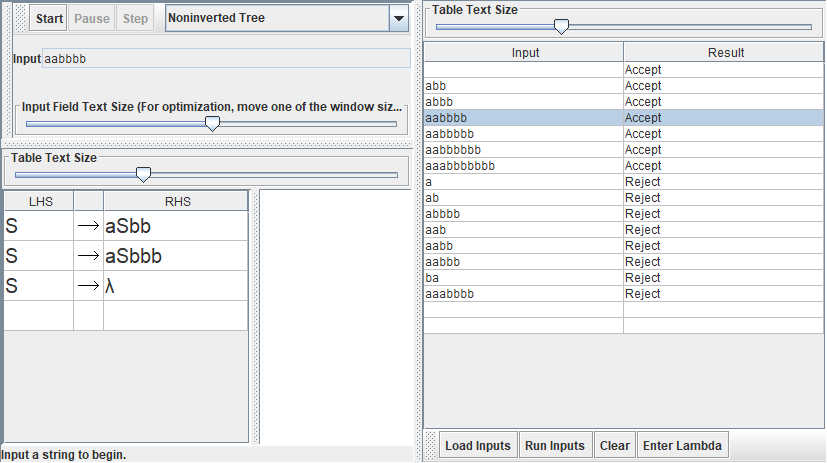
\includegraphics[width=0.95\textwidth]{Problem 1/Problem 1.png}
\caption{JFLAP verification of the grammar for Problem 1. The Multiple Run test demonstrates that the grammar correctly accepts strings where the number of $b$'s is between 2 and 3 times the number of $a$'s (such as $abb$, $abbb$, $aabbbb$, $aabbbbb$, $aabbbbbb$), and correctly rejects strings that violate this constraint (such as $a$, $ab$, $abbbb$, $aabbb$, $ba$). This empirical testing confirms the grammar generates exactly the language $L = \{a^n b^m : 2n \le m \le 3n\}$.}
\label{fig:problem1}
\end{figure}

\newpage

\subsection{Problem 2: CFG for $L = \{w \in \{a,b\}^* : n_a(w) = 2n_b(w)\}$}

\subsubsection{Problem Statement}
Create a context-free grammar for the language $L = \{w \in \{a,b\}^* : n_a(w) = 2n_b(w)\}$.

\subsubsection{Solution}

\textbf{Context-Free Grammar:}

$$S \rightarrow aabS \mid abaS \mid baaS \mid \lambda$$

\subsubsection{Explanation}

The constraint $n_a(w) = 2n_b(w)$ requires that the number of $a$'s be exactly twice the number of $b$'s. Unlike Problem 1, the symbols can appear in any order---the language allows arbitrary interleaving of $a$'s and $b$'s as long as the final count maintains the 2:1 ratio.

The grammar handles this through three recursive rules, each adding exactly 2 $a$'s and 1 $b$ in different orderings. The production $S \rightarrow aabS$ adds the pattern $aab$, while $S \rightarrow abaS$ adds $aba$, and $S \rightarrow baaS$ adds $baa$. These three rules exhaustively cover all possible local arrangements of two $a$'s and one $b$. By choosing different rules at each recursive step, the grammar can generate strings with arbitrary interleaving while maintaining the global 2:1 ratio. The base case $S \rightarrow \lambda$ generates the empty string.

\subsubsection{Sample Derivations}

\textit{Example 1: $aab$ (pattern in order)}
$$S \Rightarrow aabS \Rightarrow aab$$
Count: $n_a = 2$, $n_b = 1$, so $2 = 2(1)$ \checkmark

\textit{Example 2: $baa$ (b comes first)}
$$S \Rightarrow baaS \Rightarrow baa$$
Count: $n_a = 2$, $n_b = 1$, so $2 = 2(1)$ \checkmark

\textit{Example 3: $aabaab$ (repeated pattern)}
$$S \Rightarrow aabS \Rightarrow aabaabS \Rightarrow aabaab$$
Count: $n_a = 4$, $n_b = 2$, so $4 = 2(2)$ \checkmark

\textit{Example 4: $aabbaa$ (mixed patterns)}
$$S \Rightarrow aabS \Rightarrow aabbaaS \Rightarrow aabbaa$$
Count: $n_a = 4$, $n_b = 2$, so $4 = 2(2)$ \checkmark

\textit{Example 5: $baaaab$ (complex interleaving)}
$$S \Rightarrow baaS \Rightarrow baaaabS \Rightarrow baaaab$$
Count: $n_a = 4$, $n_b = 2$, so $4 = 2(2)$ \checkmark

\subsubsection{Formal Proof of Correctness}

\textbf{Claim:} $L(G) = \{w \in \{a,b\}^* : n_a(w) = 2n_b(w)\}$

\textbf{Proof:}

\textit{Part 1: ($L(G) \subseteq \{w \in \{a,b\}^* : n_a(w) = 2n_b(w)\}$)}

We prove by induction on the number of derivation steps that every string generated by $G$ satisfies $n_a = 2n_b$.

\textit{Base case:} If the derivation uses only $S \rightarrow \lambda$, we generate $\lambda$ with $n_a(\lambda) = 0$ and $n_b(\lambda) = 0$. Since $0 = 2(0)$, the constraint is satisfied.

\textit{Inductive hypothesis:} Assume that any string derived in $k$ or fewer steps satisfies $n_a = 2n_b$.

\textit{Inductive step:} Consider a derivation of length $k+1$. The first step must be one of: $S \rightarrow aabS$, $S \rightarrow abaS$, or $S \rightarrow baaS$.

All three productions add exactly 2 $a$'s and 1 $b$, then continue with $S$. If $S \Rightarrow^* w'$ where $n_a(w') = 2n_b(w')$ by the inductive hypothesis, then for any of the three cases:
$$n_a(\text{pattern} \cdot w') = 2 + n_a(w') = 2 + 2n_b(w') = 2(1 + n_b(w')) = 2n_b(\text{pattern} \cdot w')$$

By induction, every string in $L(G)$ satisfies $n_a = 2n_b$.

\textit{Part 2: ($\{w \in \{a,b\}^* : n_a(w) = 2n_b(w)\} \subseteq L(G)$)}

We prove by strong induction on the length of the string that every string with $n_a = 2n_b$ can be generated by $G$.

\textit{Base case:} The empty string $\lambda$ has $n_a = n_b = 0$, so $0 = 2(0)$. It is generated by $S \rightarrow \lambda$.

\textit{Inductive hypothesis:} Assume that every string of length at most $k$ with $n_a = 2n_b$ can be generated by $G$.

\textit{Inductive step:} Let $w$ be a string of length $k+1$ with $n_a(w) = 2n_b(w)$. Since $|w| > 0$ and $n_a(w) = 2n_b(w)$, we must have $n_b(w) \ge 1$ (otherwise $n_a(w) = 0$ and $w = \lambda$, contradicting $|w| > 0$).

Consider the first occurrence of $b$ in $w$. Write $w = xby$ where $x \in \{a\}^*$ and $b$ is the first $b$ in $w$. Since $n_a(w) = 2n_b(w) \ge 2$, we have $|x| \ge 2$. Therefore, we can write $x = aax'$ where $x' \in \{a\}^*$.

Now $w = aabx'y$. Let $w' = x'y$. Then:
$$n_a(w') = n_a(w) - 2 = 2n_b(w) - 2 = 2(n_b(w) - 1) = 2n_b(w')$$
and $|w'| = |w| - 3 < k+1$.

By the inductive hypothesis, $w'$ can be generated by $G$. Therefore:
$$S \Rightarrow aabS \Rightarrow^* aabw' = w$$

Thus, $w$ can be generated by $G$.

Combining both directions, we conclude that $L(G) = \{w \in \{a,b\}^* : n_a(w) = 2n_b(w)\}$. $\square$

\begin{figure}[H]
\centering
\includegraphics[width=0.95\textwidth]{Problem 2/Problem 2.png}
\caption{JFLAP verification of the grammar for Problem 2. The Multiple Run test demonstrates that the grammar correctly accepts strings with arbitrary interleaving of $a$'s and $b$'s where $n_a = 2n_b$ (such as $aab$, $aba$, $baa$, $aabaab$, $aabbaa$, $baaaab$), and correctly rejects strings that violate the 2:1 ratio (such as $a$, $b$, $ab$, $aabb$, $aaabbb$). This confirms the grammar handles all possible orderings while maintaining the constraint.}
\label{fig:problem2}
\end{figure}

\newpage

\section{Section 5.2: Derivation Trees and Ambiguity}
